% ====================================================================
%                                                                 
%
%       §07
%
%
% %%ts latex start%%[2019-03-07 Thu 14:45]%%ts latex end%%
% ====================================================================
% --------------------------------------------------------------------
% §1 Section <<Einführung>>
% --------------------------------------------------------------------
\section{Verknüpfungen}%\label{wrz}

In den Kapiteln 3 und 4 haben wir als zentrale mathematische Objekte Mengen und die Abbildungen zwischen ihnen eingeführt. Von sich aus tragen Mengen relativ wenig Information: nämlich nur, welche Elemente in ihnen enthalten sind und welche nicht. Als einen Weg, einer Menge mehr Struktur zu verleihen, wurden in Kapitel 5 Relationen thematisiert, die je zwei Elemente einer Menge in eine „Beziehung“ setzen können, wodurch die bereits aus der Schule bekannten Relationen $\leq$ und $=$ verallgemeinert wurden.

In diesem Kapitel möchten wir einen weiteren Weg, mehr Struktur in eine Menge zu bringen, vorstellen, der die bekannten Rechenoperationen wie \glqq$+$\grqq\ und \glqq$\cdot$\grqq\ verallgemeinert.

Was soll eine Verknüpfung tun? Als Input möchten wir ihr zwei Elemente $x,y$ unserer Menge geben, und als Output erwarten wir ein neues Element $z$, eben die Verknüpfung der Elemente $x$ und $y$; so wie auch die Addition „$+$“ aus zwei Zahlen $x,y$ die Zahl $z=x+y$ macht. Formal wird dies in einer Abbildung realisiert, die zwei Elemente aufnimmt und ein neues ausgibt:

\begin{de}
	Sei $X$ eine beliebige Menge. Eine (zweistellige) \textbf{Verknüpfung} auf $X$ ist eine Abbildung
		\[ X\times X \to X  \]
Eine zweistellige Verknüpung wird in der Regel mit einem „Verknüpfungszeichen“ notiert. Das heißt: ist der Name der Abbildung etwa „$*$“, so schreibt man
\[ x*y \qquad\text{anstelle von}\qquad *(x,y) \]
für den Funktionswert des Paares $(x,y)$ unter der Abbildung „$*$“.
\end{de}

\begin{bem}[*]
 Prinzipiell lassen sich auch dreistellige und höherstellige Verknüpfungen definieren. Allerdings sind so gut wie alle Verknüpfungen, die dir im Studium begegnen werden, zweistellig. Falls wir daher von „Verknüpfungen“ schreiben, sollen damit stets zweistellige Verknüpfungen gemeint sein.
\end{bem}



\begin{bsp}[Grundrechenarten]
Es gilt:
 \begin{enumerate}[a)]
 \item Auf $\Rz$ ist durch die Addition $(x,y)\mapsto x+y$ eine zweistellige Verknüpfung gegeben. Da die Summe zweier rationaler Zahlen ebenfalls rational ist, liefert „$+$“ auch eine Verknüpfung auf der Menge $\Qz$. Ebenso ist auch auf $\Nz$ und $\Zz$ durch die Addition „$+$“ jeweils eine Verknüpfung gegeben.
  \item Auf den Mengen $\Zz,\Qz,\Rz,\Cz$ ist durch die Subtraktion $(x,y)\mapsto x-y$ jeweils eine zweistellige Verknüpfung gegeben. Allerdings ergibt der Ausdruck
  \[ \text{„$\Nz \times \Nz \to \Nz \ ,\ (x,y) \mapsto x-y$“} \]
  \emph{keinen} Sinn, da etwa „$2-3$“ gar kein Element von $\Nz$ ist. Auf $\Nz$ ist die Subtraktion also \textbf{keine} zweistellige Verknüpfung. Zwar kann man für gewisse Zahlenpaare durchaus Differenzen in $\Nz$ bilden (z.B. „$3-2$“); dass „$-$“ eine Verknüpfung auf $\Nz$ wäre, scheitert aber daran, dass man eben nicht für \emph{jedes} Paar natürlicher Zahlen eine Differenz in $\Nz$ bilden kann.
  \item Auf den Mengen $\Nz,\Zz,\Qz,\Rz,\Cz$ ist durch die Multiplikation $(x,y)\mapsto x\cdot y$ jeweils eine zweistellige Verknüpfung gegeben.
  \item Auf den Mengen $\Qz\setminus \{0\},\Rz\setminus \{0\},\Cz\setminus \{0\}$ ist durch die Division $(x,y)\mapsto x:y$ jeweils eine zweistellige Verknüpfung gegeben. Beachte, dass die Null ausgelassen werden muss, weil bspw. nicht „$1:0$“ gebildet werden kann. Zwar könnte man $1:0=\infty$ setzen, aber „$\infty$“ wäre ja kein Element von $\Qz,\Rz$ bzw. $\Cz$, sodass man dadurch dennoch keine Verknüpfung auf $\Qz,\Rz$ bzw. $\Cz$ erhielte.
 \end{enumerate}
\end{bsp}





\begin{bsp}[Rechenoperationen auf Folgen]
 Auf der Menge $\Rz^\Nz$ der reellen Zahlenfolgen gibt es die folgenden Verknüpfungen, die bereits in \cref{folgenrech} eingeführt wurden:
 \begin{enumerate}[a)]
  \item Die Addition reeller Zahlenfolgen:
  \[ \Rz^\Nz\times \Rz^\Nz \to \Rz^\Nz \ ,\ ((a_n)_{n\in \Nz} , (b_n)_{n\in \Nz}) \mapsto (a_n+b_n)_{n\in \Nz} \]
  \item Die Multiplikation reeller Zahlenfolgen:
    \[ \Rz^\Nz\times \Rz^\Nz \to \Rz^\Nz \ ,\ ((a_n)_{n\in \Nz} , (b_n)_{n\in \Nz}) \mapsto (a_n\cdot b_n)_{n\in \Nz} \]
\item Ebenso kann man auch eine Subtraktion reeller Folgen definieren und, sofern man sich auf solche Folgen, in denen nirgends die Null als Eintrag auftritt, beschränkte, sogar eine Division.
 \end{enumerate}
Dies lässt sich weitreichend verallgemeinern. Wann immer auf einer Menge $X$ irgendeine Verknüpfung gegeben ist, erhält man durch „komponentenweises Verknüpfen“ eine Verknüpfung auf dem Folgenraum $X^\Nz$.
\end{bsp}





\begin{bsp}[Verkettung von Abbildungen]
 Sei $M$ eine beliebige Menge. Dann ist auf der Menge $\text{Abb}(M,M)$ der Selbstabbildungen von $M$ eine Verknüpfung gegeben durch die Verkettung\footnote{siehe \cref{verkettung}} von Abbildungen:
 \[ \text{Abb}(M,M)\times \text{Abb}(M,M)\to \text{Abb}(M,M) \ ,\ (f,g)\mapsto f\circ g \]
\end{bsp}


\begin{bem}
 Beachte, dass in diesem Beispiel von Selbstabbildungen (also Abbildungen, deren Definitions- und Wertebereich übereinstimmen) die Rede ist. Sind allgemein $A,B,C$ drei Mengen, so hat man zwar eine Abbildung
 \[ \text{Abb}(B,C) \times \text{Abb}(A,B) \to \text{Abb}(A,C) \ ,\ (f,g) \mapsto f\circ g \]
 sofern $A,B,C$ drei verschiedene Mengen sind, ist dies aber \textbf{keine} zweistellige Verknüpfung -- denn auf welcher Menge sollte diese Verknüpfung „leben“, wenn ja $\text{Abb}(B,C)$ und $\text{Abb}(A,B)$ zwei verschiedene Mengen sind? \\[0.5em]
 Nichtsdestotrotz besitzt auch das allgemeine Verketten von Abbildungen eine interessante, häufig auftretende Struktur, die man „\href{https://ncatlab.org/nlab/show/category}{Kategorie}“ nennt. Mehr darüber wirst du spätestens in fortgeschrittenen Algebra-Vorlesungen kennenlernen.
\end{bem}



\begin{bsp}[Operationen mit Mengen]
 Sei $M$ eine beliebige Menge. Dann gibt es unter Anderem die folgenden Verknüpfungen auf der Potenzmenge $\mathcal{P}(M)$:
 \begin{align*}
  \cap : \mathcal{P}(M)\times \mathcal{P}(M) \to \mathcal{P}(M) \ & ,\ (A,B)\mapsto A\cap B \\
    \cup : \mathcal{P}(M)\times \mathcal{P}(M) \to \mathcal{P}(M) \ &,\ (A,B)\mapsto A\cup B \\
\setminus : \mathcal{P}(M)\times \mathcal{P}(M) \to \mathcal{P}(M) \ &,\ (A,B)\mapsto A\setminus B
 \end{align*}
 Denn der Durchschnitt / die Vereinigung / die Differenzmenge zweier Teilmengen von $M$ ist ebenfalls eine Teilmenge von $M$.
\end{bsp}





\begin{bsp}[* Kleineres und Größeres zweier Elemente] \label{minmax}
 Sei $X$ eine beliebige totalgeordete Menge (z.B. $X=\Rz$ mit der gewöhnlichen Ordnung). Indem man von je zwei Elementen das kleinere bzw. größere auswählt, erhält man zwei Verknüpfungen auf $X$:
 \begin{align*}
  \min : X\times X\to X\ &,\ (x,y)\mapsto \min\{x,y\} \\
  \max : X\times X\to X\ &,\ (x,y)\mapsto \max\{x,y\}
 \end{align*}
Eine Verallgemeinerung sowohl dieses Beispiels als auch des Beispiels mit „$\cap$“ und „$\cup$“ stellen sogenannte „\href{https://de.wikipedia.org/wiki/Verband_(Mathematik)}{Verbände}“ dar.
\end{bsp}




\begin{bem}
Alle bisher beschriebenen Verknüpfungen besaßen ein eigenes Verknüpfungssymbol und waren relativ übersichtlich aufzuschreiben. Allgemeine Verknüpfungen auf einer Menge $X$ dürfen aber beliebig kompliziert sein. Es muss sich ja lediglich um \emph{irgendeine} Abbildung $X\times X\to X$ handeln, die beliebig chaotisch sein darf und keinem Muster gehorchen muss. Neben Addition und Multiplikation gibt es auf $\Nz$ unendlich viele weitere Verknüpfungen, von denen die meisten wohl niemals von mathematischem Interesse sein werden.
\end{bem}





\begin{bem}[Verknüpfungssymbole]
 In diesem Text werden wir, wenn wir über eine „allgemeine zweistellige Verknüpfung“ schreiben, die Verknüpfung mit einem „$*$“ notieren. Die vorigen Beispiele zeigen, dass konkrete Verknüpfungen auch mit ganz anderen Zeichen wie etwa $+,-,\cdot,:,\cap,\cup$ usw. notiert werden. Andere Bücher und Vorlesungen verwenden auch andere Symbole wie etwa „$\odot$“ oder „$\circ$“, um über „die allgemeine Verknüpfung“ zu reden. Oftmals schreiben Bücher auch gar kein Verknüpfungssymbol auf. Sind $X$ eine Menge mit einer zweistelligen Verknüpfung und $a,b\in X$ zwei Elemente, so schreiben sie einfach „$ab$“ für deren Verknüpfung, so wie du es aus der Schule auch schon von der Multiplikation zweier Zahlvariablen kennst. %\\[0.5em]
 %Fortgeschrittene Bücher notieren eine „allgemeine zweistellige Verknüpfung“ auch mit einem Multiplikationspunkt „$\cdot$“, was wir hier bewusst vermeiden, um die Verwechslungsgefahr mit der bekannten Multiplikation von Zahlen auszuschließen. \emph{Eine zweistellige Verknüpfung braucht nichts mit „Zahlen“ zu tun haben}! Oftmals schreiben solche Bücher auch gar kein Verknüpfungssymbol auf. 
\end{bem}





\section{Assoziativ- und Kommutativgesetz}


\begin{de}
 Seien $X$ eine Menge und $*$ eine Verknüpfung auf $X$. Die Verknüpfung $*$ heißt
 \begin{itemize}
  \item \textbf{assoziativ}, falls für alle $x,y,z\in X$ das sogenannte \emph{Assoziativgesetz} gilt:
  \[ x*(y*z) = (x*y)*z \]
    \item \textbf{kommutativ}, falls für alle $x,y\in X$ das sogenannte \emph{Kommutativgesetz} gilt:
  \[ x*y = y*x \]
 \end{itemize}
\end{de}





\begin{bsp}[Grundrechenarten]
 Es gilt:
 \begin{enumerate}[a)]
  \item Auf $\Nz,\Zz,\Qz,\Rz,\Cz$ sind die Addition $+$ und die Multiplikation $\cdot$ sowohl assoziativ als auch kommutativ. Denn für alle natürlichen/ganzen/rationalen/reellen/komplexen Zahlen $x,y,z$ gilt bekanntlich
  \begin{align*}
   x+(y+z)& = (x+y)+z  \\
   x+y & = y+x \\
  x\cdot (y\cdot z) & = (x\cdot y)\cdot z  \\
   x\cdot y & = y\cdot x
  \end{align*}
  \item Die Subtraktion auf $\Zz,\Qz,\Rz,\Cz$ ist weder assoziativ noch kommutativ. Beispielsweise ist
  \begin{align*}
   3-(2-1) &\neq  (3-2)-1  \\
  3-2 &\neq 2-3
  \end{align*}
\item Die Division auf $\Qz\setminus \{0\},\Rz\setminus \{0\},\Cz\setminus \{0\}$ ist weder assoziativ noch kommutativ. Beispielsweise ist
\begin{align*}
 2:(3:2) = 4:3 &\neq 1:3 = (2:3):2 \\
2 : 3 & \neq 3:2
\end{align*}
 \end{enumerate}
\end{bsp}


\begin{comment}
\begin{bsp}
 Die Grundrechenarten sind vergleichbar simple Verknüpfungen. Allgemeine Verknüpfungen dürfen aber beliebig kompliziert sein:
 \begin{itemize}
  \item Die Abbildung
  \[ \Rz_{>0}\times \Rz_{>0} \to \Rz_{>0} \ ,\ (x,y)\mapsto \frac{2xy}{x+y} \]
  ist eine zweistellige Verknüpfung auf $\Rz_{>0}$.
  \item Das \textbf{arithmetische Mittel} (umgangssprachlich „Durchschnitt“)
    \[ \Rz \times \Rz \to \Rz \ ,\ (x,y)\mapsto \frac{x+y}{2} \]
  ist eine zweistellige Verknüpfung auf $\Rz$.
 \end{itemize}
\end{bsp}
\end{comment}


\begin{bsp}[Verketten von Abbildungen] \label{verkett}
Sei $M$ eine beliebige Menge. Dann ist die Verkettung von Abbildungen eine assoziative Verknüpfung auf $\text{Abb}(M,M)$, die aber, sofern $M$ mindestens zwei Elemente enthält, nicht kommutativ ist. 
\end{bsp}
\begin{bew}[(*)]
 (Assoziativität) Dies wurde in \cref{abbass} bewiesen. \\[0.5em]
 (Nicht-Kommutativität) Die Menge $M$ enthalte mindestens zwei verschiedene Elemente $a,b\in M$. Betrachte die beiden konstanten Abbildungen
 \begin{align*}
  f_a : M\to M \ &,\ x\mapsto a \\
  f_b : M\to M \ &,\ x\mapsto b  
 \end{align*}
d.h. $f_a$ bildet jedes Element von $M$ auf $a$ ab und $f_b$ bildet alles auf $b$ ab. Dann gilt:
\begin{align*}
 (f_a\circ f_b)(a) = f_a(f_b(a)) = f_a(b)=a \neq b = f_b(a)=f_b(f_a(a))=(f_b\circ f_a)(a)
\end{align*}
Also ist $f_a\circ f_b\neq f_b\circ f_a$, sodass die Verknüpfung „$\circ$“ nicht kommutativ ist. \qed
\end{bew}






\begin{bsp}[Das Verketten von Abbildungen ist nicht kommutativ!]
 Hier ist ein weiteres, weniger abstraktes Beispiel dafür, dass das Verketten von Abbildungen im Allgemeinen nicht kommutativ ist: \\
 Betrachte die beiden Abbildungen
 \begin{align*}
  f: \Rz \to \Rz \ &,\ x\mapsto 2\cdot x \\
  g  : \Rz \to \Rz \ &,\ x\mapsto x^2
 \end{align*}
Dann gilt für jedes $x\in \Rz$:
\begin{align*}
(g\circ f)(x) & = (2\cdot x)^2 \\
(f\circ g)(x) & = 2\cdot x^2
\end{align*}
und es ist beispielsweise
\[ (g\circ f)(3)  = 36 \neq 18 = (f\circ g)(3) \]
sodass $g\circ f\neq f\circ g$ ist. Es macht einen Unterschied, ob ich erst verdoppele und dann quadriere oder erst quadriere und dann verdopple.
\end{bsp}



\begin{bsp}[Mengenverknüpfungen]
 Ist $M$ eine beliebige Menge, so sind die beiden Verknüpfungen $\cap$ und $\cup$ auf $\mathcal{P}(M)$ sowohl assoziativ als auch kommutativ. Die Operation $\setminus$ ist aber, sofern $M$ nichtleer ist, weder assoziativ noch kommutativ.
\end{bsp}
\begin{bew}
Dies ist der Inhalt von \cref{capcupgesetze}.
\end{bew}




\begin{bem}[Die tiefere Bedeutung des Assoziativgesetzes]
\label{klammerfrei}
Sei $X$ eine Menge mit einer assoziativen Verknüpfung $*$. Der tiefere Grund dafür, dass das Assoziativgesetz so eine wichtige Rolle in der Uni-Mathematik spielt, ist, dass man bei einer assoziativen Verknüpfung keine Klammern setzen braucht. Das Assoziativgesetz selbst
 \[ (x*y)*z = x*(y*z) \qquad x,y,z\in X\]
 besagt schonmal, dass bei solchen Termen, die nur drei Elemente involvieren, jede Art von Klammernplatzierung auf dasselbe Ergebnis hinausläuft. Daher kann man auch einfach
 \[ x*y*z \]
 schreiben. Mit fortgeschrittenen Techniken lässt sich beweisen, dass bei assoziativen Verknüpfungen sogar in Termen mit beliebig vielen Elementen jede Art von Klammerung auf dasselbe Ergebnis hinausläuft. Beispielsweise gilt für $a,b,c,d,e\in X$:
 \begin{align*}
  (a*(b*c))*(d*e) & =((a*b)*c)*(d*e) && (\text{Assoziativgesetz für $a$, $b$ und $c$})\\
& = (((a*b)*c)*d)*e && (\text{Assoziativgesetz für $(a*b)*c$, $d$ und $e$})  \\
  & = ((a*b)*(c*d))*e && (\text{Assoziativgesetz für $a*b$, $c$ und $d$})\\
  &=\ \text{usw.}
 \end{align*}
 Daher kann man bei assoziativen Verknüpfungen ganz allgemein überall die Klammern weglassen und in diesem Fall einfach
 \[ a*b*c*d*e \]
 schreiben. \\
 Aus der Schule bist du es ja auch gewohnt, einfach
 \[ 1+3+2+4 \qquad\text{anstelle von}\qquad (1+3)+(2+4)\ \text{oder}\ (1+(3+2))+4 \]
 zu schreiben und daran ändert sich auch an der Uni nichts. Sind beispielsweise $A,B,C,D$ vier Mengen, so schreibt man schlicht
 \[ A\cup B\cup C \cup D \]
 für deren Vereinigung, was unproblematisch ist, da $\cup$ eine assoziative Verknüpfung ist. Sind $f:A\to B$, $g:B\to C$, $h:C\to D$ drei Abbildungen, so schreibt man schlicht
 \[ h\circ g\circ f \]
 für deren Verkettung, wobei man auch hier wegen der Assoziativität keine Klammern setzen muss. \\[0.5em]
 Aber Achtung: Bei nicht-assoziativen Verknüpfungen kannst du in der Regel nicht auf Klammerung verzichten. Beispielsweise ergäbe der Ausdruck
 \[ \Rz\setminus \Qz\setminus \Rz_{>0}\]
keinen Sinn, solange du nicht klarstellst, ob
 \[ (\Rz\setminus \Qz)\setminus \Rz_{>0} \qquad\text{oder}\qquad \Rz\setminus (\Qz\setminus \Rz_{>0}) \]
 gemeint ist.
\end{bem}




\begin{comment}
\begin{bsp}[* Minimum und Maximum]
 Ist $X$ eine totalgeordnete Menge, so sind die beiden Verknüpfungen $\min$ und $\max$ aus \cref{minmax} sowohl assoziativ als auch kommutativ.
\end{bsp}
\end{comment}






\begin{comment}
\begin{bsp}[*]
 Auf jeder beliebigen Menge $X$ ist durch
 \begin{align*}
 x*y &:= y && x,y\in X  
 \end{align*}
eine Verknüpfung gegeben. Diese Verknüpfung ist assoziativ, aber, sofern $M$ mindestens zwei verschiedene Elemente enthält, nicht kommutativ.
\end{bsp}
\begin{bew}
 (Assoziativität) Seien $x,y,z\in M$ drei beliebige Elemente. Dann ist
 \[ x*(y*z) = x*z = z = (x*y)*z \]
 Also ist $*$ eine assoziative Verknüpfung. \\[0.5em]
 (Nicht-Kommutativität) Die Menge $M$ enthalte mindestens zwei verschiedene Elemente $a,b\in M$. Dann ist
 \[ a*b = b\neq a = b*a \]
 sodass die Verknüpfung nicht kommutativ ist. \qed
\end{bew}
\end{comment}




\begin{bsp}[Rechnen mit Rundungsfehlern] \label{fehlerrech}
So gut wie alle Verknüpfungen in den ersten Semestern Mathematikstudium sind assoziativ. Ein für die Informatik wichtiges Beispiel für eine nicht-assoziative Verknüpfung ist die „fehlerbehaftete Multiplikation“. Da ein Computer eine Zahl nicht mit beliebig vielen Nachkommastellen speichern kann, muss er nach solchen Rechenschritten, die die Anzahl der Nachkommastellen übers Maximum erhöhen würde, die letzte verfügbare Nachkommastelle runden. Für ein vereinfachtes Beispiel betrachte die Menge
 \[ \frac{1}{10}\Zz := \left\{ x\in \Qz \mid \exists z\in \Zz:\ x=\frac{z}{10} \right\} \]
all derjenigen rationalen Zahlen, die höchstens eine Nachkommastelle besitzen (im Dezimalsystem -- Computer würden im Binärsystem rechnen und erheblich mehr Nachkommastellen einbeziehen). Auf dieser Menge ist folgendermaßen eine zweistellige Verknüpfung „$*$“ gegeben:
\begin{quote}
 Für $a,b\in \frac{1}{10}\Zz$ bilde zuerst das gewöhnliche Produkt rationaler Zahlen $a\cdot b \in \Qz$. Runde dieses Produkt nun auf die erste Nachkommastelle. Diese gerundete Zahl sei $a*b$.
\end{quote}
Für diese Verknüpfung gilt beispielsweise:
\begin{align*}
1,5* 0,5 = 0,8 \qquad 0,1* 0,1 = 0 \qquad 2*3 = 6 \qquad 1,5 * (-0,3)= -0,5 
\end{align*}
Diese „ungenaue Multiplikation“ ist zwar kommutativ, aber nicht assoziativ, da beispielsweise:
\[ (0,1 * 0,1) * 10 = 0*10 = 0 \neq 0,1 = 0,1*1 = 0,1*(0,1*10) \qedhere \]
 \end{bsp}


 
 
 \begin{de}[Potenzen]
  Seien $X$ eine Menge mit einer assoziativen Verknüpfung $*$ und $a\in X$ irgendein Element. Für ein $n\in \Nz_{\geq 1}$ nennt man das Element, das durch $n$-faches Verknüpfen von $a$ mit sich selbst entsteht
  \[ a^n := \underbrace{a * \ldots * a}_{n\text{-mal}} \]
  (beachte, dass hier aufgrund der Assoziativität keine Klammern gesetzt werden müssen) die \textbf{$n$-te Potenz von $a$}. Beispielsweise gilt:
  \begin{align*}
   a^1 & = a \\
   a^2 & = a* a \\
   a^3 & = a*a*a \\
   a^{n+1} & = a^n*a && n\in \Nz_{\geq 1}
  \end{align*}
 \end{de}
 
 
 
 \begin{bem}\label{potlaw}
    Seien $X$ eine Menge mit einer assoziativen Verknüpfung $*$ und $a,b\in X$ mit $a*b=b*a$. Für $n,m\in \Nz_{\geq 1}$ gelten die folgenden \emph{Potenzgesetze}:
    \begin{align*}
    a^1 & = a \\
     a^{n+m} & = a^n* a^m \\
     (a^m)^n & = a^{n\cdot m} \\
    (a*b)^n &= a^n*b^n
    \end{align*}
Beachte, dass für die letzte Gleichung wichtig ist, dass $a*b=b*a$ gilt. Nur so kann man beispielsweise ohne Weiteres die Umformungen
\[ (a*b)^2 = (a*b)*(a*b) = a*(b*a)*b \overset{!}{=} a*(a*b)*b = (a*a)*(b*b) = a^2*b^2 \] 
durchführen.
 \end{bem}
\begin{bew}
 Diese Gleichungen beweist man komfortabel mit einem sogenannten \href{https://de.wikipedia.org/wiki/Vollst%C3%A4ndige_Induktion}{Induktionsbeweis}. Da diese Beweistechnik im Vorkurs nicht behandelt wurde, könntest du noch abwarten, bis sie in den ersten beiden Semesterwochen durchgenommen wurde und daraufhin nochmal hierher zurückkehren.
\end{bew}



 
 \section{Neutrales Element}


\begin{de}[Neutrales Element] \label{neutrales}
Seien $X$ eine Menge und $*$ eine zweistellige Verknüpfung auf $X$. Ein Element $e\in X$ heißt \textbf{neutrales Element}, falls für jedes $x\in X$ die folgenden beiden Gleichungen gelten:
\begin{align*}
 e*x & = x && (\text{Linksneutralität}) \\
 x*e & = x && (\text{Rechtsneutralität})
\end{align*}
\end{de}




\begin{bsp} \label{neutralbsp}
Es sei $M$ eine beliebige Menge. Dann gilt:
 \begin{enumerate}[a)]
  \item Die Addition auf $\Nz_0,\Zz,\Qz,\Rz$ bzw. $\Cz$ hat die Zahl Null als neutrales Element. Denn für jede natürliche/ganze/rationale/reelle/komplexe Zahl $x$ gilt ja
  \[ x+0=0+x=x \]
  \item Die Multiplikation auf $\Nz,\Zz,\Qz,\Rz$ bzw. $\Cz$ hat die Zahl Eins als neutrales Element. Denn für jede natürliche/ganze/rationale/reelle/komplexe Zahl $x$ ist
  \[ x\cdot 1=1\cdot x = x \]
  \item Das Verketten von Abbildungen aus $\text{Abb}(M,M)$ hat die Identität $\iden_M$ als neutrales Element. Denn für jede beliebige Abbildung $f:M\to M$ gilt
  \[ \iden_M\circ f = f\circ \iden_M = f \]
  was in \cref{idneutral} bewiesen wurde.
  \item Bezüglich der Verknüpfung $\cap$ hat $\mathcal{P}(M)$ das neutrale Element $M$. Denn es gilt:
  \begin{align*}
   A\cap M & = M\cap A = A && \text{für jede Teilmenge}\ A\subseteq M
  \end{align*}
  \item Bezüglich der Verknüpfung $\cup$ hat $\mathcal{P}(M)$ das neutrale Element $\emptyset$. Denn für jede Teilmenge $A\subseteq M$ gilt
  \[ A\cup \emptyset = \emptyset \cup A = A \]
  \item Die fehlerbehaftete Multiplikation aus \cref{fehlerrech} hat die $1$ als neutrales Element. Denn wenn ich eine rationale Zahl, die höchstens eine Nachkommastelle besitzt, mit $1$ multipliziere, ändert sich nichts, sodass auch das nachfolgende Runden nichts am Zahlenwert ändert.
  \item Hinsichtlich der Subtraktion auf $\Zz,\Qz,\Rz$ bzw. $\Cz$ gibt es \emph{kein} neutrales Element. Denn die einzige Zahl $e\in \Cz$, die
  \begin{align*}
    x-e&=x && \text{für alle}\ x\in \Zz 
  \end{align*}
  erfüllt, ist die $0$. Also käme höchstens die $0$ als neutrales Element in Betracht. Aber z.B. wegen
  \[ 0-5 \neq 5 \]
  ist die $0$ kein neutrales Element.
  \item Hinsichtlich der Division auf $\Qz\setminus \{0\},\Rz\setminus \{0\},\Cz\setminus \{0\}$ gibt es ebenfalls kein neutrales Element.
  \item Sofern $M$ eine nichtleere Menge ist, gibt es bezüglich der Verknüpfung „$\setminus$“ auf $\mathcal{P}(M)$ auch kein neutrales Element.
 %\item Hinsichtlich der Verknüpfung
 %\[ M\times M \to M \ ,\ (x,y)\mapsto y \]
 %ist jedes Element von $M$ linksneutral.
 \end{enumerate}
\end{bsp}



\begin{bem}[Beweisarbeit einsparen im kommutativen Fall]
Seien $X$ eine Menge mit einer Verknüpfung $*$ und $e\in X$ ein Element, von dem du vermutest, dass es ein neutrales Element ist. Sofern $*$ eine \emph{kommutative Verknüpfung} ist, brauchst du, um zu beweisen, dass $e$ ein neutrales Element ist, von den beiden Gleichungen
\[ e*x=x \qquad\text{und}\qquad x*e=x \qquad\qquad x\in X \]
nur eine zu beweisen. Die andere folgt dann direkt aus dem Kommutativgesetz.
\end{bem}



\begin{comment}
\begin{bsp}[* Neutrales Element bei $\min$ und $\max$]
 Sei $X$ eine totalgeordnete Menge. Dass ein Element $m\in X$ neutral bezüglich der $\max$-Verknüpfung aus \cref{minmax} ist, hieße, dass für jedes $x\in X$ gelten muss
 \[ \max \{m,x\} = x \]
 was wiederum äquivalent zu $m\leq x$ ist. Also ist ein Element genau dann neutral bezüglich $\max$, wenn es das kleinste Element von $X$ ist (sofern eines existiert). Beispielsweise wäre $0$ neutral bezüglich der $\max$-Verknüpfung auf $\Nz_0$ -- dagegen gäbe es bezüglich der $\max$-Verknüpfung auf $\Zz$ kein neutrales Element. \\
 Analog ist ein Element genau dann neutral bezüglich der $\max$-Verknüpfung, wenn es das größte Element von $X$ ist.
\end{bsp}
\end{comment}




\begin{sat}[Eindeutigkeitssatz für neutrale Elemente] \label{neutreind}
Seien $X$ eine Menge und $*$ eine Verknüpfung auf $X$, die ein neutrales Element $e\in X$ besitzt. Dann ist $e$ auch das einzige neutrale Element.
\end{sat}
\begin{bew}
Es sei $d\in X$ ein beliebiges neutrales Element bezüglich der Verknüpfung $*$. Dann gilt:
\begin{align*}
 d & = d*e && (\text{weil $e$ neutrales Element}) \\
 & = e && (\text{weil $d$ neutrales Element})
\end{align*}
Also gibt es neben $e$ keine weiteren neutralen Elemente. \qed
\end{bew}




\begin{bem}[\textbf{Das} neutrale Element]
Der Eindeutigkeitssatz berechtigt uns, beim Vorhandensein eines neutralen Elements statt von „einem neutralen Element“ von \emph{dem} neutralen Element zu reden. \\
An diesem Satz wird vielleicht deutlich, wie vorteilhaft die axiomatische Arbeit mit abstrakten Verknüpfungen sein kann. Denn er garantiert uns auf einen Schlag, dass die neutralen Elemente aus allen Beispielen in \cref{neutralbsp} auch jeweils die einzigen neutralen Elemente sind, ohne dass wir dies in jedem Fall einzeln beweisen müssten.
\end{bem}







\section{Monoide}



\begin{de}[Monoid]
 Ein \textbf{Monoid} ist ein Paar $(M,*)$ bestehend aus einer Menge $M$ und einer Verknüpfung $*$ auf $M$, für das gilt:
 \begin{enumerate}[(M1)]
  \item $*$ ist eine assoziative Verknüpfung.
  \item $M$ enthält ein neutrales Element (bezüglich der Verknüpfung $*$).
 \end{enumerate}
In diesem Fall ist das neutrale Element nach \cref{neutreind} automatisch eindeutig bestimmt. \\
 Ist überdies die Verknüpfung $*$ auch noch kommutativ, so nennt man $(M,*)$ ein \textbf{kommutatives Monoid}.
\end{de}





\begin{bsp} Es gilt:
\begin{enumerate}[a)]
 \item(Addition von Zahlen) $(\Nz_0,+),(\Zz,+),(\Qz,+),(\Rz,+),(\Cz,+)$ sind jeweils kommutative Monoide. Denn die Addition ist assoziativ und kommutativ und die Zahl $0$ ist ihr neutrales Element.
 \item(Multiplikation von Zahlen) $(\Nz,\cdot),(\Zz,\cdot),(\Qz,\cdot),(\Rz,\cdot),(\Cz,\cdot)$ sind jeweils kommutative Monoide. Denn die Multiplikation ist assoziativ und kommutativ und die Zahl $1$ ist ihr neutrales Element.
 \item Die Subtraktion und die Division liefern keine Monoide, weil sie nicht assoziativ sind. Und ein neutrales Element besitzen sie ja auch nicht.
 \item Ist $X$ eine beliebige Menge, so ist $(\text{Abb}(X,X),\circ)$ ein Monoid mit neutralem Element $\iden_X$. Sofern $X$ mindestens zwei verschiedene Elemente enthält, ist es aber nicht kommutativ, siehe \cref{verkett}
 \item Ist $X$ eine beliebige Menge, so sind $(\mathcal{P}(X),\cup)$ und $(\mathcal{P}(X),\cap)$ zwei kommutative Monoide mit den jeweiligen neutralen Elementen $\emptyset$ und $X$. Sofern $X$ nichtleer ist, ist $(\mathcal{P}(X),\setminus)$ aber kein Monoid, da es weder assoziativ ist noch ein neutrales Element enthält.
 %\item Ist $X$ eine totalgeordnete Menge, so sind $(X,\min)$ und $(X,\max)$ zwei kommutative Monoide.
 \item Die „ungenaue Multiplikation“ aus \cref{fehlerrech} besitzt zwar ein neutrales Element -- sie liefert aber kein Monoid, weil sie nicht assoziativ ist.
 \item Die Addition „$+$“ ist zwar eine assoziative Verknüpfung auf der Menge $\Nz_{\geq 1}$, aber $(\Nz_{\geq 1},+)$ ist kein Monoid, da es kein neutrales Element besitzt.
\end{enumerate}
\end{bsp}





\begin{bem}[Trägermenge]
 Beachte, dass ein Monoid immer ein Paar $(M,*)$ ist, in das sowohl die „Trägermenge“ $M$ als auch die Verknüpfung $*$ kodiert ist. Ein und dieselbe Menge kann durchaus als Trägermenge für verschiedene Monoide herhalten. Beispielsweise sind $(\Nz_0,+)$ und $(\Nz_0,\cdot)$ zwei verschiedene Monoide, die dennoch dieselbe Trägermenge $\Nz_0$ besitzen. \\
 Andererseits gibt es Mengen mit „kanonischen“ Verknüpfungen, wie z.B. $\text{Abb}(X,X)$ (wobei $X$ irgendeine Menge ist). Sprechen Mathematiker von „dem Monoid $\text{Abb}(X,X)$“, so meinen sie damit grundsätzlich das Monoid $(\text{Abb}(X,X),\circ)$, also $\text{Abb}(X,X)$ mit der Verkettung von Abbildungen als Verknüpfung. Solche Konventionen wirst du mit der Zeit durch Erfahrung und Gewohnheit verinnerlichen.
\end{bem}





\begin{bem}[Die tiefere Bedeutung des Kommutativgesetzes]
Es sei $(M,*)$ ein kommutatives Monoid. Weil dann $*$ assoziativ ist, brauchen wir nach \cref{klammerfrei} keine Klammern setzen. Sind beispielsweise $a,b,c,d\in M$, so können wir einfach
\[ a*b*c*d \]
schreiben. Das Kommutativgesetz
\begin{align*}
  x*y&=y*x && x,y\in M
\end{align*}
sagt nun aus, dass es bei der Verknüpfung \emph{zweier} Elemente nicht auf die Reihenfolge ankommt. Es lässt sich zeigen, dass es damit sogar bei der Verknüpfung beliebig vieler Elemente nicht auf die Reihenfolge ankommt. Beispielsweise gilt
\begin{align*}
 a*b*c*d & = a*c*b*d && (\text{Kommutativgesetz für $b$ und $c$}) \\
 & = c*a*b*d && (\text{Kommutativgesetz für $a$ und $c$}) \\
 & = b*d*c*a && (\text{Kommutativgesetz für $c*a$ und $b*d$}) \\
 & \text{usw.}
\end{align*}
Bei kommutativen Monoiden brauchst du also weder aufs Klammernsetzen, noch auf die Reihenfolge, in der du die Elemente verknüpfst, achten.
\end{bem}



\begin{de}[Nullte Potenz]
 Seien $(M,*)$ ein Monoid mit neutralem Element $e\in M$ und $a\in M$ irgendein Element. In \cref{potlaw} wurden bereits die $n$-ten Potenzen von $a$ für $n\in \Nz_{\geq 1}$ definiert. In Monoiden lässt sich eine „nullte Potenz“ definieren durch
 \[ a^0 := e \]
Mit dieser Definition sind die Potenzgesetze aus \cref{potlaw} allgemeiner für alle $n,m\in \Nz_0$ gültig.
\end{de}



\begin{bem}[„multiplikativ geschriebene“ Monoide]
 In fortgeschrittenen Büchern und Vorlesungen wird als Verknüpfungszeichen für ein „allgemeines Monoid $M$“ oftmals der Malpunkt „$\cdot$“ verwendet. Wir haben dies hier vermieden, damit du nicht auf die Idee kämest, ein Monoid müsse unbedingt etwas mit Zahlen und deren Multiplikation zu tun haben. \\
 Das neutrale Element notieren solche Texte dann oft mit dem Zeichen „$1$“ und nennen es das „Einselement“ des Monoids $M$. In dieser Notation gilt also
 \begin{align*}
  1\cdot x & = x \\
  x \cdot 1 & = x && x\in M
 \end{align*}
 Beachte, dass es sich hier trotz Verwendung des Zeichens „$1$“ \textbf{nicht} um die natürliche Zahl Eins handelt! Um hervorzuheben, dass es sich nicht um die Zahl Eins, sondern um das neutrale Element des Monoids $M$ handelt, kann man anstelle von „$1$“ auch „$1_M$“ schreiben.
\end{bem}





\section{Inverse Elemente}



\begin{de}[Inverse Elemente] \label{inverse}
Sei $X$ eine Menge mit einer zweistelligen Verknüpfung $*$, die ein (nach \cref{neutreind} automatisch eindeutig bestimmtes) neutrales Element $e$ besitzt. Ein Element $b\in M$ heißt \textbf{invers} zu $a$, falls es die folgenden beiden „Inversengleichungen“ erfüllt:
\begin{align*}
 b*a & = e && (\text{„$b$ ist linksinvers zu $a$“})\\
 a*b & = e && (\text{„$b$ ist rechtsinvers zu $a$“})
\end{align*}
Das Element $a$ heißt \textbf{invertierbar} (oder auch: \emph{Einheit}\footnote{Abgesehen von der Benennung hat das aber erstmal nichts mit den „Einheiten“ aus der Physik, wie z.B. „Meter“ und „Kilogramm“, zu tun.}), falls es mindestens ein zu $a$ inverses Element in $X$ gibt.
\end{de}



\begin{bem}[Keine Inversen ohne Neutrales]
Beachte, dass es nur bei Vorhandensein eines neutralen Elements überhaupt Sinn ergibt, von inversen Elementen zu sprechen. 
\end{bem}




\begin{bsp}[Addition und Multiplikation]
 Es gilt:
 \begin{enumerate}[a)]
  \item In den Monoiden $(\Zz,+),(\Qz,+),(\Rz,+),(\Cz,+)$ ist jedes Element invertierbar. Denn für jede ganze/rationale/reelle/komplexe Zahl $x$ gilt
  \begin{align*}
   x + (-x) & = 0 \\
   (-x) + x & = 0
  \end{align*}
  sodass $-x$ invers zu $x$ ist.
  \item Das einzige invertierbare Element im Monoid $(\Nz_0,+)$ ist die $0$. Denn als neutrales Element ist die $0$ invertierbar und für jede Zahl $n\in \Nz_{\geq 1}$ kann es kein $m\in \Nz_0$ mit $n+m=0$ geben.
  \item \label{inversebsp} In den Monoiden $(\Qz,\cdot),(\Rz,\cdot),(\Cz,\cdot)$ ist jedes Element $\neq 0$ invertierbar. Denn für jede rationale/reelle/komplexe Zahl $x\neq 0$ gilt
  \begin{align*}
   x \cdot \frac{1}{x} & = 1 \\
   \frac{1}{x}\cdot x & = 1
  \end{align*}
  sodass $\frac{1}{x}$ invers zu $x$ ist. Die Null ist dagegen nicht invertierbar. Denn für jede beliebige Zahl $x$ ist
  \[ 0\cdot x = 0 \neq 1 \]
 \end{enumerate}
\end{bsp}




\begin{bem}[Beweisarbeit einsparen im kommutativen Fall]
 Sei $X$ eine Menge mit einer Verknüpfung $*$, die ein neutrales Element $e\in X$ besitzt. Außerdem seien $a,b\in X$ und du vermutest, dass $b$ invers zu $a$ ist. Sofern $*$ eine \emph{kommutative} Verknüpfung ist, brauchst du, um zu beweisen, dass $b$ invers zu $a$ ist, von den beiden Gleichungen
 \[ b*a=e\qquad\text{und}\qquad a*b=e \]
 nur eine zu beweisen. Die andere folgt dann aus dem Kommutativgesetz.
\end{bem}





\begin{bem}[Das neutrale Element ist selbstinvers] \label{selbstinvers}
 Sei $X$ eine Menge mit einer zweistelligen Verknüpfung $*$, die ein neutrales Element $e\in X$ besitzt. Dann ist $e$ invertierbar und ein inverses Element zu sich selbst.
\end{bem}
\begin{bew}
 Da $e$ ein neutrales Element ist, gilt
 \[ e*e = e \]
 Und diese Gleichung entspricht beiden Inversengleichungen aus \cref{inverse} zugleich. \qed
\end{bew}




\begin{bsp}[Inverse Abbildungen]
Es gilt:
\begin{enumerate}[a)]
 \item Betrachte das Monoid $\text{Abb}(\Rz_{\geq 0},\Rz_{\geq 0})$ und darin die beiden Abbildungen
 \begin{align*}
  f : \Rz_{\geq 0}\to \Rz_{\geq 0} \ &,\ x\mapsto x^2 \\
  g: \Rz_{\geq 0}\to \Rz_{\geq 0} \ &,\ x\mapsto \sqrt{x}
 \end{align*}
Dann ist $g$ invers zu $f$.
\begin{bew}
 Für jedes $x\in \Rz_{\geq 0}$ ist
 \begin{align*}
  (f\circ g)(x) & = \sqrt{x}^2 =x = \iden_{\Rz_{\geq 0}}(x) \\
  (g\circ f)(x) & = \sqrt{x^2} = x = \iden_{\Rz_{\geq 0}}(x)
 \end{align*}
sodass bereits die Gleichheit von Abbildungen $f\circ g=\iden_{\Rz_{\geq 0}}$ und $g\circ f=\iden_{\Rz_{\geq 0}}$ gilt. Also ist $g$ invers zu $f$. \qed
\end{bew}
\item Betrachte das Monoid $\text{Abb}(\Rz,\Rz)$ und darin die Abbildung
\[ f : \Rz\to \Rz \ ,\ x\mapsto x^2 \]
Dann besitzt $f$ keine Inverse. Denn nach \cref{invkriterium} müsste dann $f$ eine bijektive Abbildung sein; aber wegen $f(1)=f(-1)$ ist $f$ nicht einmal injektiv.
\item Betrachte das Monoid $\text{Abb}(\Nz_0,\Nz_0)$ und darin die beiden Abbildungen
 \begin{align*}
  f : \Nz_0 \to \Nz_0 \ &,\ n \mapsto n+1 \\
  g: \Nz_0 \to \Nz_0 \ &,\ n\mapsto \begin{cases}
                                     0 & n=0 \\
                                     n-1 & n\geq 1
                                    \end{cases}
 \end{align*}
Dann gilt zwar $g\circ f=\iden_{\Nz_0}$. Allerdings ist $f\circ g\neq \iden_{\Nz_0}$, sodass $g$ nicht invers zu $f$ ist. Tatsächlich kann $f$ gar keine Inverse besitzen, da $f$ wegen $0\notin \im(f)$ nicht surjektiv, also erst recht nicht bijektiv, ist.
\end{enumerate}
\end{bsp}




\begin{sat}[Eindeutigkeitssatz für inverse Elemente] \label{inveind}
Seien $(M,*)$ ein Monoid und $a\in M$ ein invertierbares Element. Dann gibt es auch nur genau ein inverses Element zu $a$.\footnote{vgl. \cref{umkehreind}}
\end{sat}
\begin{bew}
 Es seien $e\in M$ das neutrale Element von $M$ und $b,b'\in X$ zwei beliebige Inverse zu $a$. Dann gilt:
 \begin{align*}
  b & = b*e && (\text{da $e$ neutral ist}) \\
  & = b* a*b' && (\text{da $b'$ invers zu $a$ ist}) \\
  %& = a'*a*a'' && (\text{Assoziativgesetz}) \\
  & = e*b' && (\text{da $b$ invers zu $a$ ist}) \\
  & = b' && (\text{da $e$ neutral ist}) \qed
 \end{align*}
\end{bew}




\begin{bem}[\textbf{Das} inverse Element]
  Seien $(M,*)$ ein Monoid und $a\in M$ ein invertierbares Element. Da dann $a$ auch nur genau ein Inverses besitzt, ergibt es Sinn, anstelle von „einem Inversen zu $a$“ von \emph{dem} Inversen von $a$ zu sprechen.
\end{bem}



\begin{bem}
 Beachte, dass wir im Beweis von \cref{inveind} implizit Gebrauch vom Assoziativgesetz gemacht haben (erkennst du, wo?). Bei einer nicht-assoziativen Verknüpfung wie z.B. der fehlerbehafteten Multiplikation aus \cref{fehlerrech}, die sowohl kommutativ ist als auch ein neutrales Element besitzt, brauchen Inverse nicht eindeutig sein. Beispielsweise gilt dort
 \begin{align*}
  0,4*2,5 & = 2,5*0,4 = 1 \\
  0,4 * 2,6 & = 2,6*0,4 = 1
 \end{align*}
sodass das Element $0,4$ mindestens zwei verschiedene Inverse besitzt, nämlich $2,5$ und $2,6$.
\end{bem}




\begin{de}[negative Potenzen]
 Seien $(M,*)$ ein Monoid mit neutralem Element $e\in M$ und $a\in M$ ein invertierbares Element mit Inversem $h\in M$. Für $n\in \Zz$ setzt man in Verallgemeinerung der bisher definierten Potenzen
 \begin{align*}
  a^n & := \begin{cases}
            \underbrace{a* \ldots * a}_{n\text{-mal}} & n \geq 1 \\
            e & n= 0 \\
            \underbrace{h * \ldots * h}_{-n\text{-mal}} & n \leq -1
           \end{cases}
 \end{align*}
Mit dieser Definition gelten in Verallgemeinerung von \cref{potlaw} für alle invertierbaren Elemente $a,b\in M$ mit $a*b=b*a$ folgende Potenzgesetze:
\begin{align*}
 a^1 & = a \\
 a^0\ & \text{ist das neutrale Element}  \\
 a^{-1}\ & \text{ist die Inverse zu $a$} \\
 a^{n+m} & = a^n*a^m \\
 (a^m)^n & = a^{n\cdot m} \\
 (a*b)^n & = a^n*b^n && n,m\in \Zz
\end{align*}
Beachte, dass die Voraussetzung $a*b=b*a$ essenziell für die letzte Gleichung ist.
\end{de}




\begin{bem}
 Ab sofort werden wir die Inverse eines invertierbaren Monoidelements $a$ meist mit „$a^{-1}$“ notieren. Viele Lehrbücher tun das auch schon von Anfang an, ohne es mit Potenzen zu motivieren.
\end{bem}







\begin{bem}[„additiv geschriebene“ Monoide]
Als Verknüpfungszeichen \emph{kommutativer} Monoide verwenden Bücher gerne ein „$+$“-Zeichen. Bis jetzt haben wir das vermieden, damit du nicht auf die Idee kommst, es müsse etwas mit der Addition von Zahlen zu tun haben. \\[0.5em]
Sofern die Verknüpfung in einem kommutativen Monoid $M$ mit „$+$“ notiert wird, ändern sich auch einige weitere Schreibweisen. Beispielsweise wird das neutrale Element dann gerne mit dem Zeichen „$0$“ notiert (es braucht aber nichts mit der Zahl Null zu tun haben!) und das „Nullelement von $M$“ genannt. Zur Abgrenzung von der natürlichen Zahl Null schreibt man manchmal auch „$0_M$“. Es gilt dann also
\begin{align*}
 x+0_M & = x && \\
 0_M + x & = x && x\in M
\end{align*}
Überdies wird für ein invertierbares Element $a\in M$ dessen Inverse nicht mit „$a^{-1}$“, sondern mit „$-a$“ notiert. Für $b\in M$ schreibt man dann
\[ b-a \qquad\text{anstelle von}\qquad b + (-a) \]
Die Inversengleichungen aus \cref{inverse} nehmen für $-a$ dann die Gestalt
\begin{align*}
 a-a & = 0 \\
 (-a) + a & = 0
\end{align*}
an, wobei die zweite Gleichung aufgrund der Kommutativität redundant ist. \\
Außerdem wird für ein $n\in \Nz_0$ (bzw. $n\in \Zz$, falls $a$ invertierbar ist) die $n$-te Potenz von $a$ nicht mit „$a^n$“, sondern mit „$n\cdot a$“ notiert. Im Fall $n\geq 1$ gilt also:
\[ n\cdot a := \underbrace{a+\ldots + a}_{n\text{-mal}} \]
Hier ist eine Gegenüberstellung der Potenzgesetze in multiplikativer und in additiver Schreibweise:
\[ \begin{tabular}{c|c r}
Multiplikative Notation & Additive Notation & $a,b\in M$,\ $n,m\in \Nz_0$\\
    \hline 
$a^1 = a$ & $1\cdot a=a$ &\\
$a^0 = 1_M$ & $0\cdot a=0_M$ &\\
$a^{-1} =$ Inverses zu $a$ & $-a =$ Inverses zu $a$& (sofern $a$ invertierbar ist) \\
$a^{n+m} = a^n\cdot a^m$ & $(n+m)\cdot a = n\cdot a + m\cdot a$ & \\
$(a^m)^n = a^{n\cdot m}$ & $n\cdot (m\cdot a) = (n\cdot m)\cdot a$ & \\
$(a\cdot b)^n =a^n\cdot b^n$ & $n\cdot (a+b) = n\cdot a+n\cdot b$ & (sofern $a\cdot b=b\cdot a$ ist)
   \end{tabular} \]
   \begin{comment}
\begin{align*}
 1 \cdot a & = a \\
 0_{\Nz}\cdot a & = 0_M \\
 (-1)\cdot a & = -a && (\text{sofern $a$ invertierbar ist})\\
 (n+m) \cdot a & = n\cdot a + m\cdot a \\
 (n\cdot m) \cdot a & = n\cdot (m\cdot a) \\
 n\cdot (a+b) & = n\cdot a + n\cdot b && a,b\in M,\ n,m\in \Nz_0
\end{align*}
\end{comment}
Beachte, dass es sich hierbei um ein- und dieselbe Sache, nur in zwei verschiedenen Schreibweisen, handelt.
\end{bem}








\begin{sat}[Regel von Hemd und Jacke]
Seien $(M,*)$ ein Monoid und $a,b\in M$ zwei invertierbare Elemente. Dann ist auch $a*b$ invertierbar und es gilt
\[ (a*b)^{-1} = b^{-1} * a^{-1} \]
Beim Invertieren dreht sich also die Reihenfolge um.
\end{sat}
\begin{bew}
 Es gilt
 \begin{align*}
  b^{-1}*a^{-1} * a*b  & =  b^{-1} * e* b && \\
  & = b^{-1} * b \\
  & = e
 \end{align*}
sowie
  \begin{align*}
 a*b* b^{-1}*a^{-1}  & =  a*e*a^{-1} && \\
  & = a*a^{-1} \\
  & = e
 \end{align*}
Insgesamt erfüllt $b^{-1}*a^{-1}$ somit beide Inversengleichungen. \qed
\end{bew}





\begin{bem}
 Dieser Satz wird „Regel von Hemd und Jacke“ genannt aufgrund folgender Analogie: Habe ich mir erst ein Hemd und daraufhin eine Jacke angezogen und möchte mich nun wieder entkleiden -- so muss ich zuerst die Jacke und dann das Hemd ausziehen. \\[0.5em]
Im kommutativen Fall kommt es nicht auf die Reihenfolge an, sodass man dann auch $(a*b)^{-1} = a^{-1}*b^{-1}$ schreiben kann. Insofern ist dir die Regel von Hemd und Jacke gar nicht fremd: schließlich hast du auch in der Schule regelmäßig benutzt, dass:
\begin{align*}
 -(x+y) & = -x -y && x,y\in \Rz \\
 \frac{1}{x\cdot y} &= \frac{1}{x}\cdot \frac{1}{y} && x,y\in \Rz\setminus \{0\}
\end{align*}
\end{bem}




\begin{sat}[Inverses vom Inversen] \label{doppelinvers}
Seien $(M,*)$ ein Monoid und $a\in M$ ein invertierbares Element. Dann ist auch $a^{-1}$ invertierbar und es gilt
\[ (a^{-1})^{-1} = a \]
\end{sat}
\begin{bew}
Sei $e\in M$ das neutrale Element von $M$. Da $a^{-1}$ invers zu $a$ ist, gelten die beiden Gleichungen
\[ a*a^{-1} = e \qquad\text{und}\qquad a^{-1}*a=e \]
Die erste dieser Gleichungen besagt, dass $a$ linksinvers zu $a^{-1}$ ist und die zweite Gleichung besagt, dass $a$ rechtsinvers zu $a^{-1}$ ist. Insgesamt ist also $a$ die Inverse von $a^{-1}$. \qed
\end{bew}


\begin{bem}
 Auch diese Regel ist dir in Spezialfällen aus der Schule bekannt. Schließlich gilt
 \begin{align*}
  -(-x) & = x && x\in \Rz \\
  \frac{1}{\frac{1}{x}} & = x && x\in \Rz\setminus \{0\}
 \end{align*}
\end{bem}





\section{Gruppen}

\begin{de}[Gruppe]
Eine \textbf{Gruppe} ist ein Monoid, in dem jedes Element invertierbar ist. Konkret handelt es sich bei einer Gruppe also um ein Paar $(G,*)$ bestehend aus einer Menge $G$ und einer Verknüpfung $*$ auf $G$, für das die sogenannten \emph{Gruppenaxiome} gelten:
\begin{enumerate}[(G1)]
 \item Die Verknüpfung $*$ ist assoziativ.
 \item $G$ enthält ein neutrales Element (bezüglich der Verknüpfung $*$).
 \item Jedes Element von $G$ ist invertierbar.
\end{enumerate}
Ist überdies die Verknüpfung auch noch kommutativ, so spricht man von einer \textbf{abelschen Gruppe}\footnote{\href{https://de.wikipedia.org/wiki/Niels_Henrik_Abel}{Niels Henrik Abel (1802-1829)}}.
\end{de}





\begin{bsp}
 Es gilt:
 \begin{enumerate}[a)]
  \item $(\Zz,+),(\Qz,+),(\Rz,+),(\Cz,+)$ sind jeweils abelsche Gruppen. Denn die Addition ist assoziativ, kommutativ, besitzt die $0$ als neutrales Element und für jede ganze/rationale/reelle/komplexe Zahl $x$ ist $-x$ ebenfalls eine ganze/rationale/reelle/komplexe Zahl und invers zu $x$.
  \item Das Monoid $(\Nz_0,+)$ ist keine Gruppe, da beispielsweise das Element $5\in \Nz_0$ nicht invertierbar ist.
%  \item $(\Qz\setminus \{0\},\cdot),(\Rz\setminus \{0\},\cdot),(\Cz\setminus \{0\},\cdot)$ sind jeweils abelsche Gruppen.
 % \item Sofern $X$ eine nichtleere Menge ist, sind die Monoide $(\mathcal{P}(X),\cap)$ und $(\mathcal{P}(X),\cup)$ keine Gruppen.
  \item Sofern $X$ eine mindestens zweielementige Menge ist, ist das Monoid $\text{Abb}(X,X)$ keine Gruppe.
\begin{bew}[(*)]
 Seien $a\in X$ irgendein Element und $f:X\to X$ die konstante Abbildung, die alles auf $a$ abbildet. Weil $X$ mindestens zwei Elemente enthält, ist $f$ injektiv und nach \cref{invkriterium} somit auch nicht invertierbar in $\text{Abb}(X,X)$. Also ist $\text{Abb}(X,X)$ keine Gruppe. \qed
\end{bew}
 \end{enumerate}
\end{bsp}



\begin{comment}
\begin{bsp}[*]
	Als ein Beispiel neben den Zahlenräumen betrachten wir einmal die Symmetrien eines Vierecks:
	\begin{figure}[h]
		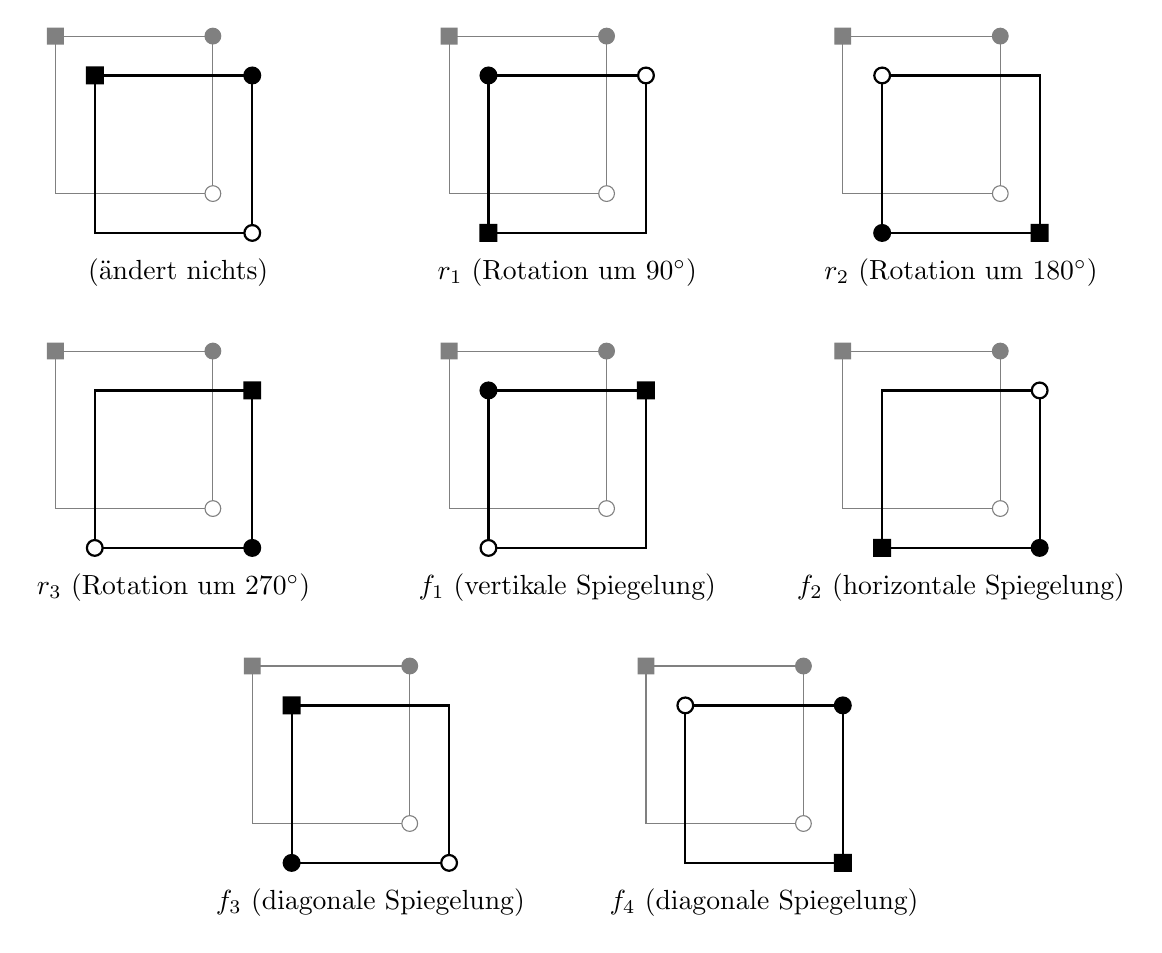
\begin{tikzpicture}
			
		\foreach \xtext / \xangle / \xshift /\yshift in
			{
			$\iden$ (ändert nichts)/0/-5cm/3cm,
			$r_1$ (Rotation um $90^\circ$)/90/0cm/3cm,
			$r_2$ (Rotation um $180^\circ$)/180/5cm/3cm,
			$r_3$ (Rotation um $270^\circ$)/270/-5cm/-1cm
			}
			{
			\begin{scope}[xshift=\xshift, yshift=\yshift]
				\begin{scope}[xshift=-.5cm,yshift=.5cm,gray,thin]
				\draw (0,0) rectangle (2,2);
				\filldraw (-.1,1.9) rectangle (.1,2.1) (2,2) circle (.1cm);
				\filldraw[fill=white, draw=gray] (2,0) circle (.1cm);
			\end{scope}
			\begin{scope}[thick, rotate around={\xangle:(1,1)}]
				\draw (0,0) rectangle (2,2);
				\filldraw (-.1,1.9) rectangle (.1,2.1) (2,2) circle (.1cm) (2,0);
				\filldraw[fill=white, draw=black] (2,0) circle (.1cm);
			\end{scope}
			\path (1,-.2) node[below] {\xtext};
			\end{scope}
			};
			
		\foreach \xtext / \xscale / \yscale / \xangle / \xshift / \yshift / \xxshift / \yyshift in
			{
				$f_1$ (vertikale Spiegelung)/-1/1/0/0cm/-1cm/-2cm/0cm,
				$f_2$ (horizontale Spiegelung)/1/-1/0/5cm/-1cm/0cm/-2cm,
				$f_3$ (diagonale Spiegelung)/-1/1/270/-2.5cm/-5cm/-2cm/0cm,
				$f_4$ (diagonale Spiegelung)/-1/1/90/2.5cm/-5cm/-2cm/0cm
			}
			{
				\begin{scope}[xshift=\xshift, yshift=\yshift]
					\begin{scope}[xshift=-.5cm,yshift=.5cm,gray,thin]
						\draw (0,0) rectangle (2,2);
						\filldraw (-.1,1.9) rectangle (.1,2.1) (2,2) circle (.1cm);
						\filldraw[fill=white, draw=gray] (2,0) circle (.1cm);
					\end{scope}
					\begin{scope}[thick, xscale=\xscale,yscale=\yscale, xshift=\xxshift, yshift=\yyshift, rotate around={\xangle:(1,1)} ]
						\draw (0,0) rectangle (2,2);
						\filldraw (-.1,1.9) rectangle (.1,2.1) (2,2) circle (.1cm) (2,0);
						\filldraw[fill=white, draw=black] (2,0) circle (.1cm);
					\end{scope}
					\path (1,-.2) node[below] {\xtext};
				\end{scope}
			};
			
		\end{tikzpicture}
	\centering \caption{Symmetrien eines Quadrates}
	\end{figure}
	
	Auf der Menge $S=\{\iden,r_1,r_2,r_3,f_1,f_2,f_3,f_4\}$ betrachten wir die Hintereinanderausführung von Abbildungen $\circ$ als Verknüpfung; etwa gilt $f_1\circ f_2=r_2$, wie man sich mittels eines Bildchens schnell verdeutlicht. Die Verkettung zweier Symmetrien ergibt wieder eine Symmetrie, also ist $\circ$ tatsächlich eine Verknüpfung auf $S$. [Tabelle?]
	
	Wir möchten nun zeigen, dass $(S,\circ,\iden)$ eine Gruppe bildet, und prüfen dazu die geforderten Eigenschaften.
	Dass $\circ$ assoziativ ist, gilt ganz allgemein für Abbildungen [Referenz?].
	Die Identität $\iden$ ist neutrales Element bezüglich $\circ$, siehe [Referenz].
	Jetzt müssen wir noch zu jedem Element Inverse finden. Die Identität hat als Inverses sich selbst, denn es gilt
		\[ \iden\circ\iden=\iden \,.\]
	Die Rotation um $x$ Grad hat als Inverses die Rotation um $360-x$ Grad (denn Hintereinanderausführung ergibt dann die Rotation um 360 Grad, die der Identität entspricht). Konkret:
		\begin{align*}
			r_1\circ r_3 &= \iden = r_3\circ r_1 \,, \\
			r_2\circ r_2 &= \iden \,.
		\end{align*}
	Führt man dieselbe Achsenspiegelung zwei mal hintereinander aus, landen man wieder, wo man gestartet ist, also sind die vier Achsenspiegelungen alle selbstinvers:
		\[ \iden=f_1\circ f_1=f_2\circ f_2=f_3\circ f_3 = f_4\circ f_4\,. \]
		
	Damit ist bewiesen, dass $(S,\circ,\iden)$ eine Gruppe ist.
\end{bsp}
\end{comment}



Viele interessante Verknüpfungen liefern lediglich Monoide aber keine Gruppen. Allerdings kann aus jedem Monoid eine (mehr oder weniger große) Gruppe extrahiert werden, indem man sich einfach auf die invertierbaren Elemente einschränkt:


\begin{de}[Einheitengruppe eines Monoids]
Sei $(M,*)$ ein Monoid. Die Teilmenge
\[ M^\times := \{x\in M\mid x\ \text{ist invertierbar} \} \]
heißt die \textbf{Einheitengruppe} von $M$.
\end{de}


\begin{sat} \label{einheitengruppe}
 Sei $(M,*)$ ein Monoid. Dann kann die Verknüpfung von $M$ auf $M^\times$ eingeschränkt werden. Auf diese Weise wird $M^\times$ zu einer Gruppe. Ist $M$ ein kommutatives Monoid, so ist $M^\times$ eine abelsche Gruppe.
\end{sat}
\begin{bew}
(Einschränkbarkeit) Nach der Regel von Hemd und Jacke ist für alle $a,b\in M^\times$ auch $a*b\in M^\times$. Somit liefert $*$ durch Einschränkung eine zweistellige Verknüpfung auf der Menge $M^\times$. \\[0.5em]
(Assoziativität): Da $*$ eine assoziative Verknüpfung ist, gilt
\begin{align*}
 x*(y*z) & = (x*y)*z && x,y,z\in M
\end{align*}
Also gilt diese Gleichung auch erst recht für alle Elemente von $M^\times$. Somit ist $*$ auch auf $M^\times$ eine assoziative Verknüpfung. \\[0.5em]
(Neutrales Element): Sei $e\in M$ das neutrale Element von $M$. Nach \cref{selbstinvers} ist $e\in M^\times$. Weil für alle $x\in M$ gilt
\[ e*x=x*e=x \]
gilt dies erst recht auch für alle $x\in M^\times$. Somit ist $e$ ein neutrales Element in $M^\times$. \\[0.5em]
(Inverse): Sei $a\in M^\times$. Dann ist $a$ ein invertierbares Element von $M$. Nach \cref{doppelinvers} ist auch $a^{-1}$ invertierbar, also $a^{-1}\in M^\times$. Wegen
\begin{align*}
 a*a^{-1}=a^{-1}*a=e
\end{align*}
und weil $e$ das neutrale Element in $M^\times$ ist, ist dann $a^{-1}$ auch in $M^\times$ invers zu $a$. \\[0.5em]
(Kommutativität) Sei $M$ ein kommutatives Monoid. Dann gilt für alle $x,y\in M$:
\[ x*y=y*x \]
Also gilt diese Gleichung erst recht auch für alle Elemente von $M^\times$, sodass $M^\times$ in diesem Fall eine abelsche Gruppe ist. \qed
\end{bew}







\begin{bsp}
Es gilt:
\begin{itemize}
 \item Die Einheitengruppe des Monoids $(\Nz_0,+)$ ist $\{0\}$. Insbesondere ist $(\{0\},+)$ eine Gruppe, die nur ein einziges Element enthält. Solche Gruppen nennt man auch \emph{triviale Gruppen}.\footnote{vgl. \cref{verkbsp}d)}
 \item Die Einheitengruppe des Monoids $(\Zz,\cdot)$ ist $\{1,-1\}$. Insbesondere ist $(\{1,-1\},\cdot)$ eine Gruppe, die aus genau zwei Elementen besteht.
 \item Nach \cref{inversebsp} ist die Einheitengruppe des Monoids $(\Rz,\cdot)$ genau $\Rz\setminus \{0\}$. Somit ist $(\Rz\setminus \{0\},\cdot)$ eine Gruppe.
\end{itemize}
\end{bsp}




\begin{de}[Permutationsgruppe]
 Sei $M$ eine beliebige Menge. Die Menge der bijektiven Selbstabbildungen von $M$
 \[ S(M) := \{f\in \text{Abb}(M,M)\mid f\ \text{ist bijektiv} \} \]
 heißt die \textbf{symmetrische Gruppe} von $M$. Ihre Elemente heißen \textbf{Permutationen} von $M$.
\end{de}


\begin{sat}
 Sei $M$ eine Menge. Dann ist $S(M)$ mit der Verkettung von Abbildungen als Verknüpfung eine Gruppe. Es handelt sich genau um die Einheitengruppe von $\text{Abb}(M,M)$.
\end{sat}
\begin{bew}
 Aus \cref{invkriterium} folgt, dass eine Abbildung $f:M\to M$ genau dann bijektiv ist, wenn sie invertierbar im Monoid $\text{Abb}(M,M)$ ist. Also ist $S(M)$ tatsächlich die Einheitengruppe von $\text{Abb}(M,M)$ und nach \cref{einheitengruppe} somit eine Gruppe. \qed
\end{bew}




\begin{bem}[Endliche Permutationsgruppen]
 Für eine Zahl $n\in \Nz_0$ schreibt man
 \[ S_n := S(\{1,\dots , n\}) \]
 für die Permutationsgruppe der Menge $\{1,\dots , n\}$. Diese Gruppen sind von großer Bedeutung in der Gruppentheorie, da sie nach dem sogenannten „\href{https://de.wikipedia.org/wiki/Satz_von_Cayley}{Satz von Cayley}“ in einem gewissen Sinne „universell“ sind unter allen Gruppen, die nur endlich viele Elemente besitzen. Die $S_n$-Gruppen werden dir bereits in der LA1-Vorlesung wieder begegnen, dort spätestens im Kontext von \emph{Matrixdeterminanten}.
\end{bem}




\begin{bem}[* Grothendieck\footnote{\href{https://de.wikipedia.org/wiki/Alexander_Grothendieck}{Alexander Grothendieck (1928-2014)}}-Gruppe]
 Neben dem Konzept „Einheitengruppe“ gibt es ein weiteres Rezept, um aus Monoiden Gruppen zu machen: die sogenannte „\href{https://de.wikipedia.org/wiki/Grothendieck-Gruppe}{Grothendieck-Gruppe}“. Während man, um von einem Monoid zu seiner Einheitengruppe zu gelangen, die Trägermenge soweit verkleinert, bis nur noch die invertierbaren Elemente übrigbleiben, fügt man bei der Grothendieck-Gruppe „künstliche Inverse“ hinzu. Beispielsweise kann die Gruppe $(\Zz,+)$ dadurch konstruiert werden, dass man dem Monoid $(\Nz_0,+)$ für jedes $n\in \Nz_0$ eine „künstliche Inverse $-n$“ beilegt. Auch die Zahlbereichserweiterung $\Zz \mapsto \Qz$ geschieht durch die Hinzufügung künstlicher Inverser, diesmal bezüglich der Multiplikation. Solche Techniken, bei denen man für eine Struktur gewisse wünschenswerte Eigenschaften künstlich erzwingt, sind typisch für die abstrakte Algebra und tauchen dort beispielsweise bei den Konzepten „Quotientenkörper“, „Lokalisierung eines Rings“, „Tensoralgebra“ oder „Zerfällungskörper“ auf.
\end{bem}






\newpage
\section{Aufgabenvorschläge}




\begin{aufg} \label{verkbsp}
Entscheidet für jede der folgenden Verknüpfungen, ob sie assoziativ ist, kommutativ ist, ob sie ein neutrales Element besitzt und ob sie ein Monoid oder gar eine Gruppe liefert. Sofern ein Monoid vorliegt, bestimmt dessen Einheitengruppe.
\begin{enumerate}[a)]
 \item Die auf der Menge $\Nz_0$ durch
 \[ \Nz_0 \times \Nz_0 \to \Nz_0 \ ,\ (n,m) \mapsto n^m \]
 gegebene Verknüpfung (wobei $n^0=1$ für alle $n\in \Nz_0$ sei).
 \item Auf der Menge $\Rz_{>0}$ der positiven reellen Zahlen die Multiplikation $(x,y)\mapsto x\cdot y$.
 \item Die auf der Menge $\Rz$ durch
 \[ \Rz\times \Rz \to \Rz \ ,\ (x,y) \mapsto 96 \]
 gegebene Verknüpfung (d.h. je zwei beliebige Elemente verknüpfen sich immer zu $96$).
\item Auf einer beliebigen einelementigen Menge eine beliebige zweistellige Verknüpfung.
 \item Es sei $V$ die Gesamtheit aller Mengen. Betrachte darauf die Verknüpfung
 \[ V\times V\to V \ ,\ (A,B) \mapsto \{A,B\} \]
\end{enumerate}
\end{aufg}




\begin{aufg}
Seien $(M,*)$ ein Monoid und $a\in M$ ein invertierbares Element. Beweist, dass „Multiplikation mit $a$“ eine Äquivalenzumformung ist, d.h. dass für alle $x,y\in M$ gilt:
\begin{align*}
x&=y \quad \leftrightarrow\quad a*x=a*y \\
x&=y \quad \leftrightarrow\quad x*a=y*a
\end{align*}
Gilt dies auch, wenn $a$ nicht invertierbar ist? Könnt ihr ein Gegenbeispiel für diesen Fall finden?
\end{aufg}





\begin{aufg}
Sei $X$ eine beliebige Menge. Beweist die Äquivalenz der folgenden Aussagen:
\begin{enumerate}[(i)]
 \item Die symmetrische Gruppe $S(X)$ ist eine abelsche Gruppe.
 \item $X$ enthält höchstens zwei verschiedene Elemente.
\end{enumerate}
\end{aufg}



\begin{aufg}
Sei $X$ irgendeine Menge.
\begin{enumerate}[a)]
 \item Beweist, dass die Einheitengruppe des Monoids $(\mathcal{P}(X),\cup)$ aus nur einem einzigen Element besteht. Welchem?
 \item Beweist, dass das Monoid $(\mathcal{P}(X),\cup)$ dann und nur dann eine Gruppe ist, wenn $X=\emptyset$.
\end{enumerate}
\end{aufg}
\begin{comment}
\subsection{Aufgabe}
Sei $X$ eine beliebige Menge. Es bezeichne
\[ \text{Rel}(X) := \{{\sim}\mid {\sim}\ \text{ist eine zweistellige Relation auf $X$} \} \]
die Menge aller Relationen auf $X$. Für zwei Relationen ${\sim_1},{\sim_2}\in \text{Rel}(X)$ sei die Relation „$\sim_1\land \sim_2$“ definiert durch
\begin{align*}
 x\ (\sim_1 \land \sim_2)\ y  \qquad:\Leftrightarrow\qquad x\sim_1 y\ \text{und}\ x\sim_2 y && x,y\in X
\end{align*}
\begin{enumerate}[a)]
 \item Sei $X=\Rz$. Bestimmt die Relation $\sim_1\land \sim_2$ in den folgenden drei Fällen:
 \begin{align*}
  {\sim_1} = \text{„$\leq$“} \quad \text{und}\quad {\sim_2} = \text{„$\geq$“} \\
  {\sim_1} = \text{„$\leq$“} \quad \text{und}\quad {\sim_2} = \text{„$\neq$“} \\
  {\sim_1} = \text{„$<$“} \quad \text{und}\quad {\sim_2} = \text{„$>$“} 
 \end{align*}
\item Zeigt, dass $(\text{Rel}(X),\land)$ ein kommutatives Monoid ist. Was ist das neutrale Element?
\end{enumerate}





\begin{aufg}[* Große Abschlussaufgabe (nur für Profis)] \label{abschlussaufgabe}
Diese Aufgabe beinhaltet Konzepte aus nahezu allen Vorkursvorträgen. Komm eventuell nochmal in ein paar Wochen hierher zurück, wenn du dich besser an diese Denkweisen gewohnt hast.\\[0.5em]
Es sei
\[ \mathcal{A} := \{ A\mid A\ \text{ist eine Aussage} \} \]
die Menge aller Aussagen. Betrachtet darauf die folgende Relation „$\sim$“:
\begin{align*}
A\sim B\qquad &:\Leftrightarrow\qquad \text{Es lässt sich beweisen, dass $A\leftrightarrow B$ gilt}  && A,B\in \mathcal{A} 
\end{align*}
Nach \cref{aussagenequiv} ist „$\sim$“ eine Äquivalenzrelation auf $\mathcal{A}$. Die zugehörige Faktormenge bezeichnen wir mit „$L$“\footnote{Man nennt $L$ die \emph{Lindenbaum-Algebra}}:
\[ L := \{ k\subseteq\mathcal{A} \mid k\ \text{ist eine Äquivalenzklasse bezüglich}\ {\sim} \} \]
\begin{enumerate}[a)]
 \item Beweist, dass es auf der Menge $L$ genau eine Relation „$\leq$“ gibt, bei der für alle $A,B\in \mathcal{A}$ gilt:
 \[ [A]\leq [B]\qquad\Leftrightarrow\qquad \text{Es lässt sich beweisen, dass $A\to B$ gilt} \]
Zeigt außerdem, dass „$\leq$“ eine Ordnungsrelation, also reflexiv, transitiv und antisymmetrisch, ist.
\item Beweist, dass es eindeutig bestimmte zweistellige Verknüpfungen „$\land$“ und „$\lor$“ auf $L$ gibt, die für alle $A,B\in \mathcal{A}$ die folgenden Gleichungen erfüllen:
\begin{align*}
[A]\land [B] & = [A\land B] \\
[A]\lor [B] & = [A\lor B]
\end{align*}
\item Beweist, dass in der geordneten Menge $(L,\leq)$ jede zweielementige Menge ein Infimum und ein Supremum besitzt. Um genau zu sein, dass für alle $x,y\in L$ gilt:
\[ \inf \{x,y\} = x\land y \qquad\text{und}\qquad \sup \{x,y\} = x\lor y \]
\item Sei $E$ eine beliebige Eigenschaft. Zeigt, dass die Menge $\{ [E(a)] \mid a\ \text{ist irgendein Objekt} \}$ jeweils ein Infimum und ein Supremum in $L$ besitzt. Um genau zu sein:
\begin{align*}
\inf \{ [E(a)] \mid a\ \text{ist ein Objekt} \}&= [ \forall x: E(x)]  \\
\sup \{ [E(a)] \mid a\ \text{ist ein Objekt} \} & =  [ \exists x: E(x)] 
\end{align*}
\item Zeigt, dass $(L,\land)$ und $(L,\lor)$ jeweils kommutative Monoide sind.
\end{enumerate}
\end{aufg}
\end{comment}


\begin{comment}
Auf der Menge $\Rz^\Nz$ der reellen Zahlenfolgen wurde im letzten Vortrag\footnote{siehe \cref{folgenrech}} eine Addition eingeführt:
\[ + : \Rz^\Nz\times \Rz^\Nz\to \Rz^\Nz \ ,\ ((a_n)_{n\in \Nz} , (b_n)_{n\in \Nz} )\mapsto (a_n+b_n)_{n\in \Nz} \]
\begin{enumerate}[a)]
 \item Beweist, dass $(\Rz^\Nz,+)$ eine Gruppe ist, indem ihr nacheinander die Gruppenaxiome durchgeht.
 \item Sei nun $(G,*)$ eine beliebige Gruppe. Auf der Menge $G^\Nz$ der $G$-wertigen Folgen lässt sich die Verknüpfung
 \[ * : G^\Nz\times G^\Nz\to G^\Nz \ ,\ ((g_n)_{n\in \Nz} , (h_n)_{n\in \Nz} )\mapsto (g_n* h_n)_{n\in \Nz} \]
 definieren. Beweist, dass $(G^\Nz,*)$ eine Gruppe ist.
 \item Macht euch klar, dass a) ein Spezialfall von b) ist. Lässt sich die Aussage aus b) noch weiter verallgemeinern?
\end{enumerate}
\end{comment}








\begin{comment}
\newpage
\section{Elementare Eigenschaften}

%------------------
% 1.1 Def. Gruppe
\begin{de}[(abelsche) Gruppe]
Sei $G$ eine  nicht-leere Menge, $e\in G$ ein (ausgezeichnetes) Element und 
\[
 *\colon G\times G \to G
\]
eine Abbildung.
Wir nennen das Tripel $(G,*,e)$ eine \swdde{Gruppe}, falls für beliebige $a,b,c\in G$ gilt
\begin{enumerate}[\colde\upshape(i)]
\item $(a*b)*c=a*(b*c)$ \hfill (Assoziativität)
\item $a*e=a$ \hfill (Ex. rechtsneutrales El.)
\item Es gibt $d\in G$ mit $a*d=e$ \hfill (Ex. rechtsinverses El.)
\end{enumerate}
wir nennen die Gruppe zusätzlich \swdde{abelsch}, falls gilt
\begin{enumerate}[\colde\upshape(iv)]
\item $a*b=b*a$ \hfill (Kommutativität)
\end{enumerate}
%\deEnd
\end{de}

%------------------
% 1.2 Bsp. Gruppe
\begin{bsp}
\begin{bspListeN}[]%\leavevmode%
\item $(\Zz,+,0)$ ist eine abelsche Gruppe
\item $(\Qz\backslash\{0\},\cdot,1)$ ist eine abelsche Gruppe
\item $(\{-1,1\},\cdot,1)$ ist eine abelsche Gruppe
\item $(\Nz, \cdot, 1)$ ist keine Gruppe
\end{bspListeN}
\end{bsp}

%------------------
% 1.3 Bsp. Gruppe
\begin{bsp}
Wir betrachten die Menge der bijektiven Abbildungen $M=\{1,2,3\} \ra M$
\begin{align*}
S_3=\{e=\id[3],\;
d_1=(1 \,2\, 3),\;
d_2=(1\, 3\, 2),\;
\tau_1=(2\,3),\;
\tau_2=(1\,3),\;
\tau_3=(1\,2)\}
\end{align*}\
Als erstes fällt uns auf, dass für $f,g\in S_3\colon f \circ g \in S_3$.
Z.\,B.: $d_1 \circ \tau_1=(1\,2)=\tau_3\in S_3$ oder $\tau_1 \circ d_1=(1\,3)\in S_3$.
Insbesondere gilt hier also nicht die Kommutativität.
\\
Außerdem gilt für $f,g,h\in S_3\colon(f\circ g)\circ h=f \circ(g\circ f)$, denn es gilt für $x\in M$ beliebig:
\begin{align*}
	((f\circ g)\circ h)(x) &\overset{\text{Def}}{=} (f\circ h)(h(x)) \overset{\text{Def}}{=} f(g(h(x))) \\
	(f\circ(g\circ h))(x) &= f((g\circ h)(x)) = f(g(h(x))) 
\end{align*}
Also gilt die behauptete Gleichheit. \\
Da $e\in S_3$ jedes Element wieder auf sich selber abbildet, gilt für $f\in S_3\colon f\circ e=f$.
\\
Außerdem können jede dieser Abbildungen wieder umkehren:
\[
	e\circ e=e,\; d_1\circ d_2=e,\; d_2\circ d_1=e\; \tau_1\circ \tau_1=e,\;\tau_2 \circ \tau_2=e\;\tau_3\circ \tau_3=e
\]

Insgesamt handelt es sich bei $S_3$ also um eine Gruppe.
\\
Wenn wir nun die bijektiven Abbildungen $S_n$ von $M_n=\{1, \dots, n\}$ für $n\geq 3$ betrachten, fällt uns auf, dass diese auch nicht-abelsche Gruppen sind.
Deshalb betrachten wir jetzt Gruppen, als Verallgemeinerung dieses Konzeptes, um Aussagen über all diese Mengen zu treffen.
\end{bsp}


% --------------------------------------------------------------------
% §2 Section <<Elementare Eigenschaften>>
% --------------------------------------------------------------------







%\label{pot}

%------------------
% 2.1 Lemma
\begin{lem}
Sei $G$ eine Gruppe, $a,b\in G$, s.\,d., $a*b=e$. Dann gilt auch $b*a=e$, $b$ ist also auch ein linksinverses El. von $a$.
\end{lem}

%------------------
% 2.2 Beweis
\begin{bew}
Sei $c \in G$ rechtsinvers von $b$, also $b*c=e$.
Dann gilt:
\[
	b*a \overset{\text{1ii}}{=} (b*a)*e \overset{b*c=e}{=} (b*a)*(b*c) \overset{\text{1i}}{=} b*(a*b)*c \overset{a*b=e}{=} b*e*c \overset{\text{1ii}}{=} b*c \overset{n.V}{=} e.
\]
\bewEnd
\end{bew}

%------------------
% 2.3 Lemma
\begin{lem}
Sei $G$ eine Gruppe, dann ist $e\in G$ auch linksneutral, also für $a\in G\colon e*a=a$.
\end{lem}

%------------------
% 2.4 Beweis
\begin{bew}
Sei $a \in G$ bel. und $b\in G$, s.\,d., $a*b=e$. Dann gilt:
\[
	e*a \overset{\text{n.\,V.}}{=} (a*b)*a \overset{\text{1i}}{=} a*(b*a) \overset{\text{4}}{=} a*e \overset{\text{1ii}}{=} a
\]
\bewEnd
\end{bew}

%------------------
% 2.5 Lemma
\begin{lem}
Sei $G$ eine Gruppe. Dann ist $e$ das einzige neutrale Element, d.\,h., für $\tilde{e}\in G$ ein neutrales Element gilt bereits $e=\tilde{e}$.
\end{lem}

%------------------
% 2.6 Beweis
\begin{bew}
Es gilt $e=e*\tilde{e}=\tilde{e}$
\bewEnd
\end{bew}

%------------------
% 2.7 Lemma
\begin{lem}
Sei $G$ eine Gruppe, $a\in G$. Dann gilt es nur ein zu $a$ inverses Element.
D.\,h., für $b,c\in G$ mit $a*b=e=a*c$ gilt bereits $b=c$ 
\end{lem}

%------------------
% 2.8 Beweis
\begin{bew}
Es ergibt sich
\[
	b\overset{\text{5}}{=}e*b\overset{\text{n.\,V.}}{=}(c*a)*b\overset{\text{1i}}{=}c*(a*b)\overset{\text{n.\,V.}}{=}c*e\overset{\text{1ii}}{=}c
\]
\bewEnd
\end{bew}

%------------------
% 2.9 Bem.
\begin{bem}
Wir haben bis jetzt gesehen, dass ein rechtsneutrales Element auch ein linksneutrales Element ist und es nur ein Element mir dieser Eigenschaft gibt.
Dieses Element nennen wir das \swdde{neutrale Element}.

Außerdem ist ein rechtsinverses Element auch ein linksinverses Element und zu jedem $a\in G$ gibt es genau ein $b\in G$ mit dieser Eigenschaft.
Wir nennen dieses Element das \swdde{inverse Element von $a$} und wir schreiben $a^{-1}:=b$.
Insbesondere gilt $(a^{-1})^{-1}=a$.
\bemEnd
\end{bem}

%------------------
% 2.10 Lemma Kuerzungsregel
\begin{lem}[Kürzungsregel]
Sei $G$ eine Gruppe. $a, b, c \in G$ mit $a*b = a * c$. Dann gilt $b = c$
\end{lem}

%------------------
% 2.11 Beweis
\begin{bew}
Seien $a, b, c \in G$ wie oben, dann gilt:
\[
	b\overset{\text{5}}{=}e*b\overset{\text{1iii}}{=}(a^{-1}*a)*b\overset{\text{1ii}}{=}a^{-1}*(a*b)\overset{\text{n.\,V.}}{=}a^{-1}*(a*c)\overset{\text{1i}}{=}(a^{-1}*a)*c \overset{\text{1i/iii}}{=} c
\]
\bewEnd
\end{bew}






% --------------------------------------------------------------------
% §3 Section <<Untergruppen und Nebengruppen>>
% --------------------------------------------------------------------
\section{Untergruppen und Nebengruppen}%\label{pot}

%------------------
% 3.1 Def. Untergruppe
\begin{de}%\label{defi::12}
Sei $G$ eine Gruppe und $H\subseteq G$ nicht-leer. Wir nennen $H$ eine \swdde{Unterguppe} von $G$, falls für alle $a,b\in H$ gilt
\begin{enumerate}[\colde\upshape(i)]
\item $a*b \in H$
\item $a^{-1}\in H$
\end{enumerate}
\deEnd
\end{de}

%------------------
% 3.2 Beispiel Untergruppen
\begin{bsp}
\begin{bspListeN}[]
\item $2\Zz = \{2a \mid a \in \Zz\}\subseteq\Zz$ ist eine Untergruppe
\item $\{\pm 1\} \subseteq \Qz$ ist eine Untergruppe
\item Für $G$ eine Gruppe, ist $\{e\}\subseteq G$ eine Untergruppe
\item $A_3=\{e,d_1,d_2\}\subseteq S_3$ ist eine Untergruppe (sogar abelsch)
\end{bspListeN}
\end{bsp}

%------------------
% 3.3 Lemma
\begin{lem}
Seien $G$ Gruppe, $H\subseteq G$ Untergruppe.
Dann gilt $e\in H$ und $(H,*_{|H},e)$ mit der auf $H$ eingeschränkten Verknüpfung selbst eine Gruppe.
Gilt zusätzlich $G$ abelsch, dann ist $H$ abelsch.
\end{lem}

%------------------
% 3.4 Beweis
\begin{bew}
$H$ ist nicht-leer, also gibt es $a\in  H$. Damit ist $a^{-1}\in H$ nach 10ii.
Dann gilt $e=a*a^{-1}\in H$ nach 10i.
\begin{enumerate}
\item[(0)] Wohldefiniertheit: es muss gelten $\forall a,b \in H : a*b\in H$, dies gilt nach 10i
\item Assoziativ: Seien $a,b,c\in H$, dann gilt $a,b,c\in G$, also gilt
\[
	(a*b)*c=a*(b*c)
\]
\item Rechtsneutrale Element: Es ist $e\in H$ und für $a\in H\colon a*e=a$
\item Inverses Element: folgt aus 10ii
\item Kommutativität: falls G abelsch ist, gilt für $a,b\in H\colon a*b=b*a$ in $G$, also auch in $H$ 
\end{enumerate}
\bewEnd
\end{bew}

%------------------
% 3.5 Lemma
\begin{lem}
Sei $G$ Gruppe, $H\subseteq G$, $e\in H$, $(H,*,e)$ Gruppe. Dann gilt $H\subseteq G$ Untergruppe.
\end{lem}

%------------------
% 3.6 Beweis
\begin{bew}
\begin{bewListeN}
\item gilt, da $H$ wohldefiniert
\item folgt aus 1(iii)
\end{bewListeN}
\bewEnd
\end{bew}

%------------------
% 3.7 Bem.
\begin{bem}
$G$ eine Gruppe, $a\in G$. Für $n\in\Zz$ definieren wir:
\begin{align*}
a^n:=
\begin{cases}
\underbrace{a*a*\cdots *a}^{n\text{-mal}} & n>0\\
e & n=0\\
\underbrace{a^{-1}*a^{-1}*\cdots *a^{-1}}_{(-n)\text{-mal}} & n<0,
\end{cases}
\end{align*}
es gilt
\[
\langle a \rangle := \{a^n| n\in \Zz \} \subseteq G
\]
ist eine Untergruppe. Wir nennen diese, die \swdde{von $a$ erzeugte Untergruppe}.
\end{bem}

%------------------
% 3.8 Beweis
\begin{bew}
Übungsaufgabe
\bewEnd
\end{bew}

%------------------
% 3.9 Def. 
\begin{de}%\label{defi::17}
$G$ Gruppe, $H\subseteq G$ Untergruppe. Wir definieren eine Relation auf $G$ via
\[
	a\sim_H b :\lrP a^{-1}b \in H
\]
\deEnd
\end{de}

%------------------
% 3.10 Beispiel
\begin{bsp}
Wir betrachten $G = \Zz$ und $H = 2\Zz$.
Für $a, b \in \Zz$ erhalten wir also
\[
	a \sim b \lrP b - a \in 2\Zz
\]
Also muss die Differenz von $a$ und $b$ gerade sein.
Das ist genau dann der Fall, wenn $a$ und $b$ beide gerade sind oder beide ungerade sind.
\bspEnd
\end{bsp}

%------------------
% 3.11 Lemma
\begin{lem}%\label{lemm::18}
Die Relation aus \cref{defi::17} ist eine Äquivalenzrelation.
\end{lem}

%------------------
% 3.12 Beweis
\begin{bew}
Seien $a,b,c\in G$ beliebig
\begin{enumerate}
\item Reflexiv: $a^{-1}a=e\in H$, also $a\sim_H a$
\item Symmetrie: Gelte $a\sim_H b$, also $a^{-1}b\in H$\\
Es gilt $(b^{-1}a) = (a^{-1}b)^{-1}$, denn:
\[
	(a^{-1}b)(b^{-1}a)= a^{-1} *(bb^{-1})*a=a^{-1}a=e
\]
Also $ b^{-1}a =(a^{-1}b)^{-1} \in H$, folgt aus \cref{defi::12}ii, also $b\sim_H a$
\item Transitiv:
Gelte $a\sim_H b$ und $b\sim_H c$. Dann gilt $$ a^{-1}c = a^{-1} (bb^{-1}) c=
\underbrace{(a^{-1} b)}_{\in H} \underbrace{(b^{-1}c)}_{\in H} \in H$$
also $a\sim_H c$
\end{enumerate}
\end{bew}

%------------------
% 3.13 Lemma
\begin{lem}%\label{lemm::19}
$G$ Gruppe $H\subseteq G$ UG, $a\in G$.
Dann ist die Äquivalenzklasse von $a$ bzgl $\sim_H$ gegeben durch
\[
	[a]=aH:=\{ah\mid h\in H\}
\]
\end{lem}

%------------------
% 3.14 Beweis
\begin{bew}
\begin{bewListeN}[]
\item[\glqq$\subseteq$\grqq] Sei $b \in [a]$, also $a \sim b$, also $a^{-1}*b = h \in H$. Damit erhalten wir
\[
	b = (aa^{-1})b = a(\underbrace{a^{-1}b}_{= h}) = ah
\]
Also $b \in aH$.
\item[\glqq$\supseteq$\grqq] Sei $b \in aH$, also $b = ah$ für $h \in H$. Wir erhalten
\[
	a^{-1}b = a^{-1}ah = h \in H
\]
Also $a \sim b$ und $b \in [a]$.
\end{bewListeN}
\end{bew}

%------------------
% 3.15 Notation
\begin{sch}
Wir schreiben
\[
	G/H := G/\sim_H = \{[a] \mid a \in G\}
\]
\end{sch}

%------------------
% 3.16 Beispiel
\begin{bsp}
$\Zz/2\Zz = \{\{\ldots,-4,-2,0,2,4,\ldots\}, \{\ldots,-5,-3,-1,1,3,5,\ldots\}\}$
\end{bsp}


% --------------------------------------------------------------------
% §4 Section <<Der Satz von Lagrange>>
% --------------------------------------------------------------------
\section{Der Satz von Lagrange}

%------------------
% 4.1 Def. 
\begin{de}
Sei $G$ eine Gruppe. Wir nennen $G$ \swdde{endlich}, falls die Menge $G$ nur endlich viele Elemente besitzt.
Sei $H \subseteq G$ eine Untergruppe. Ist $G/H$ eine endliche Menge, so nennen wir
\[
	(G:H) := \#(G/H)
\]
den \swdde{Index von $H$ in $G$}.

Sei $a \in G$. Wir definieren die \swdde{Ordnung} von $a$ durch
\[
	\ord(a) := \min\{n\in \NN \mid a^n = e\} \qquad \text{wobei } \min\emptyset := \infty
\]
\deEnd
\end{de}

%------------------
% 4.2 Bem.
\begin{bem}
Sei $G$ eine Gruppe, $a \in G$. Dann gilt
\[
	\ord(a) = \#\langle a \rangle
\]
\end{bem}

%------------------
% 4.3 Beweis
\begin{bew}
Übungsaufgabe
\bewEnd
\end{bew}

%------------------
% 4.4 Lemma
\begin{lem}
Sei $G$ eine Gruppe, $H \subseteq G$ eine Untergruppe. Dann gilt
\begin{enumerate}
\item Je zwei Äquivalenzklassen sind gleichmächtig
\item Je zwei Äquivalenzklassen sind disjunkt oder gleich
\item $G$ ist die disjunkte Vereinigung der Äquivalenzklassen
\end{enumerate}
\end{lem}

%------------------
% 4.5 Beweis
\begin{bew}
\begin{enumerate}
\item Es genügt für $a \in G$ bel zu zeigen, dass $\#[a] = \#[e]$.
Dafür betrachten wir $f\colon H \ra aH, h \mapsto ah$. $f$ ist injektiv, denn seien $h_1, h_2 \in H$ mit $f(h_1) = f(h_2)$ dann gilt
\[
	ah_1 = f(h_1) = f(h_2) = ah_2 \overset{\text{9}}{\rP} h_1 = h_2
\]
Da $f$ injektiv ist, gilt nun $\#[a] \geq \#[e]$.

Außerdem ist $f$ surjektiv, denn sei $b = ah \in aH$. Dann gilt
\[
	b = f(h)
\]
Damit ist $\#[a] \leq \#[e]$.

Also muss bereits $\#[a] = \#[e]$ gelten. Damit folgt nun für $a, b \in G$ beliebig
\[
	\#[a] = \#[e] = \#[b]
\]
\item folgt da $\sim$-Äquivalenzrelation
\item folgt da $\sim$-Äquivalenzrelation
\end{enumerate}
\end{bew}

%------------------
% 4.6 Satz von Lagrange
\begin{sat}[Lagrange]
Sei $G$ eine endliche Gruppe, $H \subseteq G$ eine Untergruppe. Dann gilt:
\[
	\#G = \#H \cdot (G:H)
\]
\end{sat}

%------------------
% 4.7 Beweis
\begin{bew}
Wir schreiben zunächst
\[
	G/H = \{[a_1], \ldots, [a_n]\}
\]
mit disjunkten $[a_1], \ldots, [a_n]$ (Lemma 23ii) und $n = \# G/H = (G:H)$ (Definition 21). Wir haben
\[
	G = \mathop{\overset\bullet\bigcup} \limits _ {i=1,\ldots,n} [a_i] \qquad \text{Lemma 23iii}
\]
und damit folgt
\[
	\# G = \# \left(\mathop{\overset\bullet\bigcup} \limits _ {i=1,\ldots,n} [a_i]\right) = \sum \limits _{i=1}^n \#[a_i] \overset{\text{23}}{=} \sum \limits _{i=1}^n \#[e] = n \cdot \# [e] = (G:H) \cdot \# H
\]
\bewEnd
\end{bew}

%------------------
% 4.8 Korollar
\begin{kor}
Sei $G$ eine endliche Gruppe, $a \in G$. Dann gilt $\ord(a) | ord(G)$ bzw.
\[
	a^{\#G} = e
\]
\end{kor}
\end{comment}

% --------------------------------------------------------------------
% §5 Section <<Übungsaufgaben>>
% --------------------------------------------------------------------






%%% Local Variables:
%%% mode: latex
%%% TeX-master: "Skript"
%%% End:
